\documentclass[11pt]{article}
\usepackage[a4paper,margin=22mm]{geometry}
\usepackage{graphicx}
\usepackage{booktabs}
\usepackage{array}
\usepackage{amsmath}
\usepackage{xcolor}
\usepackage{hyperref}
\usepackage{caption}
\usepackage{float}
\usepackage{microtype}
\hypersetup{colorlinks=true,linkcolor=blue!45!black,urlcolor=blue!55!black,citecolor=blue!45!black}
\captionsetup{font=small,labelfont=bf}
\setlength{\parindent}{0pt}
\setlength{\parskip}{0.55em}
\newcommand{\good}[1]{\textcolor{green!40!black}{\textbf{#1}}}
\newcommand{\caution}[1]{\textcolor{orange!65!black}{\textbf{#1}}}
\newcommand{\negative}[1]{\textcolor{red!60!black}{\textbf{#1}}}

\title{Metabolic-gene-only structure in a 3CA meningioma single-cell RNA-seq dataset\\
\large Reproducible analysis report (Q1\_R18)}
\author{Automated analysis of Weizmann Curated Cancer Cell Atlas data}
\date{14 September 2026}

\begin{document}
\maketitle

\begin{abstract}
This report tests whether a user-supplied list of 1,988 metabolic genes defines transcriptional states in a single 3CA study with enough annotated cell diversity and exact CD8 T-cell labels. The selected dataset is Choudhury \emph{et al.} 2022 (meningioma; 10x; 58,843 cells, 10 samples, 6 patients). Of the supplied symbols, 1,798 matched the dataset, and 1,415 passed the global prevalence filter. Metabolic-gene-only clustering produced a six-cluster global partition after a prespecified 5\% minimum-cluster-size guardrail. However, its separation was modest, sensitive to initialization, and worse than every one of 19 expression-matched random non-metabolic gene sets. The clusters were associated with cell type, but patient, sample, and transcript-complexity associations were of comparable magnitude, so a metabolism-specific interpretation is not supported. In 3,624 CD8 T cells, no solution from $k=2$ to $8$ met the 5\% size rule. The apparent two-cluster solution isolated only 54 cells, 45 of them from patient 1, with approximately seven-fold higher median detected-gene complexity. The defensible conclusion is therefore: candidate transcriptional groupings exist, but this dataset does not establish distinct, metabolism-specific states globally or robust, replicated metabolic states within CD8 T cells.
\end{abstract}

\section{Direct answers}

\begin{table}[H]
\centering
\small
\begin{tabular}{>{\raggedright\arraybackslash}p{0.29\textwidth}>{\raggedright\arraybackslash}p{0.17\textwidth}>{\raggedright\arraybackslash}p{0.46\textwidth}}
\toprule
Question & Answer & Evidence and interpretation \\
\midrule
(1) Are there distinct clusters using metabolic genes only? & \negative{Not established} & A valid global $k=6$ partition had silhouette $0.213$, but mean adjusted Rand index (ARI) across four alternate seeds was only $0.527$ (minimum $0.423$). On the matched control subsample, all 19 random non-metabolic gene sets separated cells at least as well (empirical add-one $p=1.00$). Thus clustering is possible, but it is not specific evidence for metabolic-state structure. \\
\addlinespace
(2) Are the clusters associated with cell type? & \caution{Yes, descriptively; confounded} & Normalized mutual information (NMI) was $0.354$ for cell type and $0.476$ for cell subtype. Yet NMI was also $0.407$ for patient and $0.361$ for sample. Cluster median complexity varied from 1,088.5 to 5,481.5 detected genes. Cell identity, patient composition, and technical/global transcriptional complexity can therefore explain much of the structure. \\
\addlinespace
(3) Are there different states within CD8 T cells? & \negative{No robust evidence} & No $k=2\ldots8$ solution met the 5\% minimum-cluster rule. The best unconstrained split was 54 versus 3,570 cells; 45 of the 54 cells came from patient 1, and no patient contained both clusters at $\geq5\%$. This is a reproducible rare outlier group, not a replicated CD8 metabolic state. \\
\bottomrule
\end{tabular}
\caption{Answers are deliberately phrased at the level supported by the data. ``Not established'' does not mean that metabolic states are biologically absent; it means that this analysis cannot distinguish them from other sources of transcriptional structure.}
\end{table}

\section{Data source and provenance}

The Weizmann Curated Cancer Cell Atlas (3CA) homepage was queried on 14 September 2026. At retrieval, the homepage reported 124 studies, 2,836 samples, and 5,658,705 cells. The machine-readable catalog contained 124 unique citations and reported 2,838 samples and 5,658,779 cells; this small portal/catalog mismatch is recorded rather than silently reconciled. The study was selected after refreshing the 3CA catalog and reviewing a T-cell search plus the available study metadata. A single-study design was used to avoid making cross-study batch effects the primary clustering signal.

\begin{table}[H]
\centering
\small
\begin{tabular}{ll}
\toprule
Field & Value \\
\midrule
3CA study & Choudhury \emph{et al.} 2022 (3CA ID 20773) \\
Disease / tissue & Meningioma / brain \\
Technology & 10x single-cell RNA sequencing \\
Cells / samples / patients & 58,843 / 10 / 6 \\
Cell types & Malignant, monocyte, T cell, pericyte, endothelial, glia \\
Exact CD8 T-cell subtype & 3,624 cells across 10 samples and 6 patients \\
Expression matrix & 33,538 genes $\times$ 58,843 cells; 177,192,137 non-zero entries \\
User metabolic list & 1,988 unique symbols; 1,798 matched; 190 unmatched \\
\bottomrule
\end{tabular}
\caption{Study and gene-list scope. Sample count is not treated as independent patient count because several samples are regions from the same patient.}
\end{table}

\begin{minipage}{\textwidth}\small\raggedright
The downloaded data archive had SHA-256
\texttt{2156a73f\allowbreak d5f95a19\allowbreak 8ef90821\allowbreak f2d734bf\allowbreak a7e0b5aa\allowbreak 3686deef\allowbreak d1b5c5d5\allowbreak d1269aa1}; the metadata archive had SHA-256
\texttt{0614f546\allowbreak a5691606\allowbreak 6ed8f7fc\allowbreak a1a24dbd\allowbreak fc9e7b28\allowbreak af1bd1c9\allowbreak e982a59a\allowbreak 25ea3828}. Both archives passed the 3CA manifest verification before analysis. The user gene-list file had SHA-256
\texttt{7503180d\allowbreak 29693bd1\allowbreak e654ea93\allowbreak 281db0e3\allowbreak ec4177ff\allowbreak 44842c8b\allowbreak 02f6a098\allowbreak 402e41a9}.
\end{minipage}

\section{Analysis design}

\subsection{Preprocessing}

Raw UMI counts from the verified 3CA archive were used. Each cell was normalized by its total library size to 10,000 counts and transformed with $\log(1+x)$. Only exact, case-normalized symbols from the supplied list were eligible. Within each analysis scope, a gene had to be detected in at least 1\% of cells, with a minimum of 20 cells. This retained 1,415 genes globally and 1,214 genes in CD8 T cells. Eligible genes were centered, scaled to unit variance, and clipped to $[-10,10]$. Randomized principal component analysis (PCA) and clustering used these metabolic genes only; cell annotations were introduced only after clustering. Global partitions used mini-batch $k$-means, whereas the smaller CD8 scope used standard $k$-means; both used 20 initializations per fit.

\subsection{Clustering and guardrails}

The number of clusters was searched over a prespecified range: $k=2\ldots12$ globally and $k=2\ldots8$ in CD8 T cells. The primary solution maximized silhouette score among partitions whose smallest cluster contained at least 5\% of the relevant cells. If no candidate met this rule, the unconstrained optimum was retained only as a diagnostic result and explicitly marked invalid for primary interpretation. This guardrail prevents a tiny outlier population from being presented as a general metabolic state.

Stability was evaluated by comparing the seed-0 solution with seeds 17, 42, 73, and 101 using ARI. Silhouette calculations used a fixed seed and a bounded cell subsample where needed. To test gene-set specificity, 19 random non-metabolic gene sets were approximately matched to the metabolic genes on detection prevalence and mean count, then processed using the same cells, gene count, PCA, and selected $k$. The empirical add-one value was
\[
 p_{\mathrm{emp}}=\frac{1+\#\{S_{\mathrm{random}}\geq S_{\mathrm{metabolic}}\}}{1+19}.
\]
With only 19 controls, the smallest possible value is 0.05; these values are exploratory calibration, not confirmatory hypothesis tests.

\subsection{Annotation association and statistical unit}

NMI and adjusted mutual information (AMI) quantify descriptive association between unsupervised clusters and 3CA annotations. They do not prove causation or biological mechanism. Patient is the relevant independent biological unit; individual cells are nested measurements. Consequently, this report does not convert tens of thousands of cells into pseudo-replicated $P$-values. Per-patient composition and per-patient cell-type NMI are reported to reveal heterogeneity. No external cohort was used, so all cluster labels and gene signatures remain exploratory.

\section{Results}

\subsection{Question 1: metabolic-gene-only clustering}

The unconstrained global silhouette optimum was $k=5$, but its smallest cluster contained only 2.19\% of cells. Under the prespecified 5\% rule, $k=6$ was selected. The six clusters contained 5,519--17,736 cells each (9.38--30.14\% of the dataset). The silhouette score was $0.213$, indicating modest separation. The first 10 metabolic PCs explained only 11.36\% of variance. Across alternate initializations, mean ARI was $0.527$ and the minimum was $0.423$, indicating substantial sensitivity of the exact partition.

Most importantly, the metabolic list did not outperform matched genes. On the common control subsample, the metabolic-gene silhouette was $0.290$, whereas every one of 19 matched random non-metabolic lists gave an equal or higher score (range visually shown in Fig.~\ref{fig:global-evidence}); the add-one empirical value was 1.00. This directly argues against calling the observed separation metabolism-specific.

\begin{figure}[H]
\centering
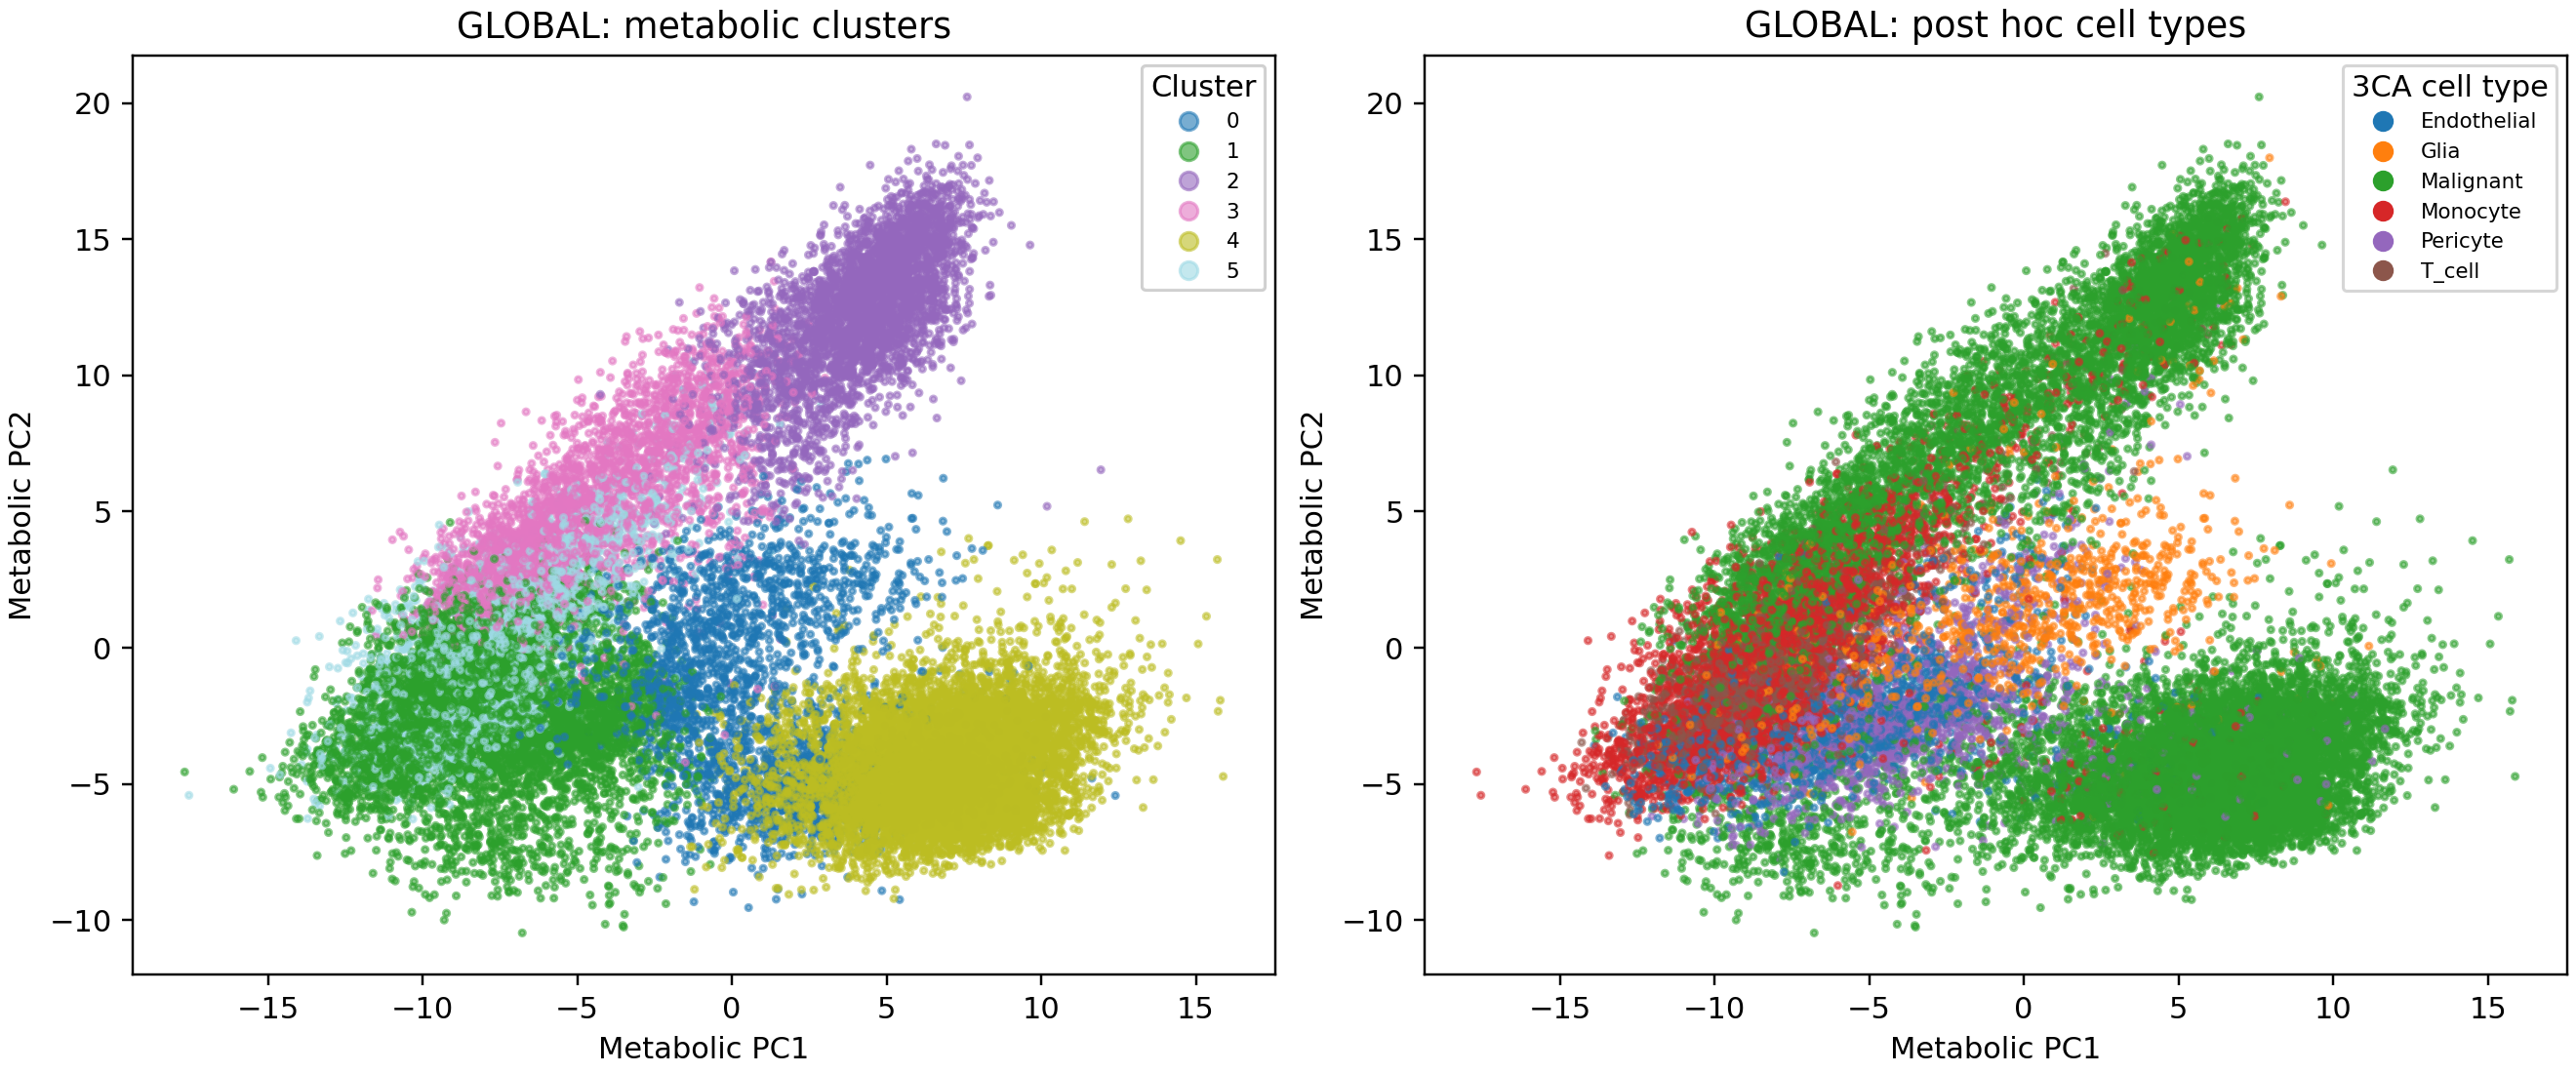
\includegraphics[width=\textwidth]{../figures/global_embedding.png}
\caption{Global metabolic-gene PCA. Left: six-cluster partition selected after the 5\% minimum-cluster rule. Right: the same PCA coordinates colored post hoc by 3CA cell type. Annotation was not used to construct the PCA or clusters. The visual overlap and gradients argue against sharply separated universal states.}
\label{fig:global-embedding}
\end{figure}

\begin{figure}[H]
\centering
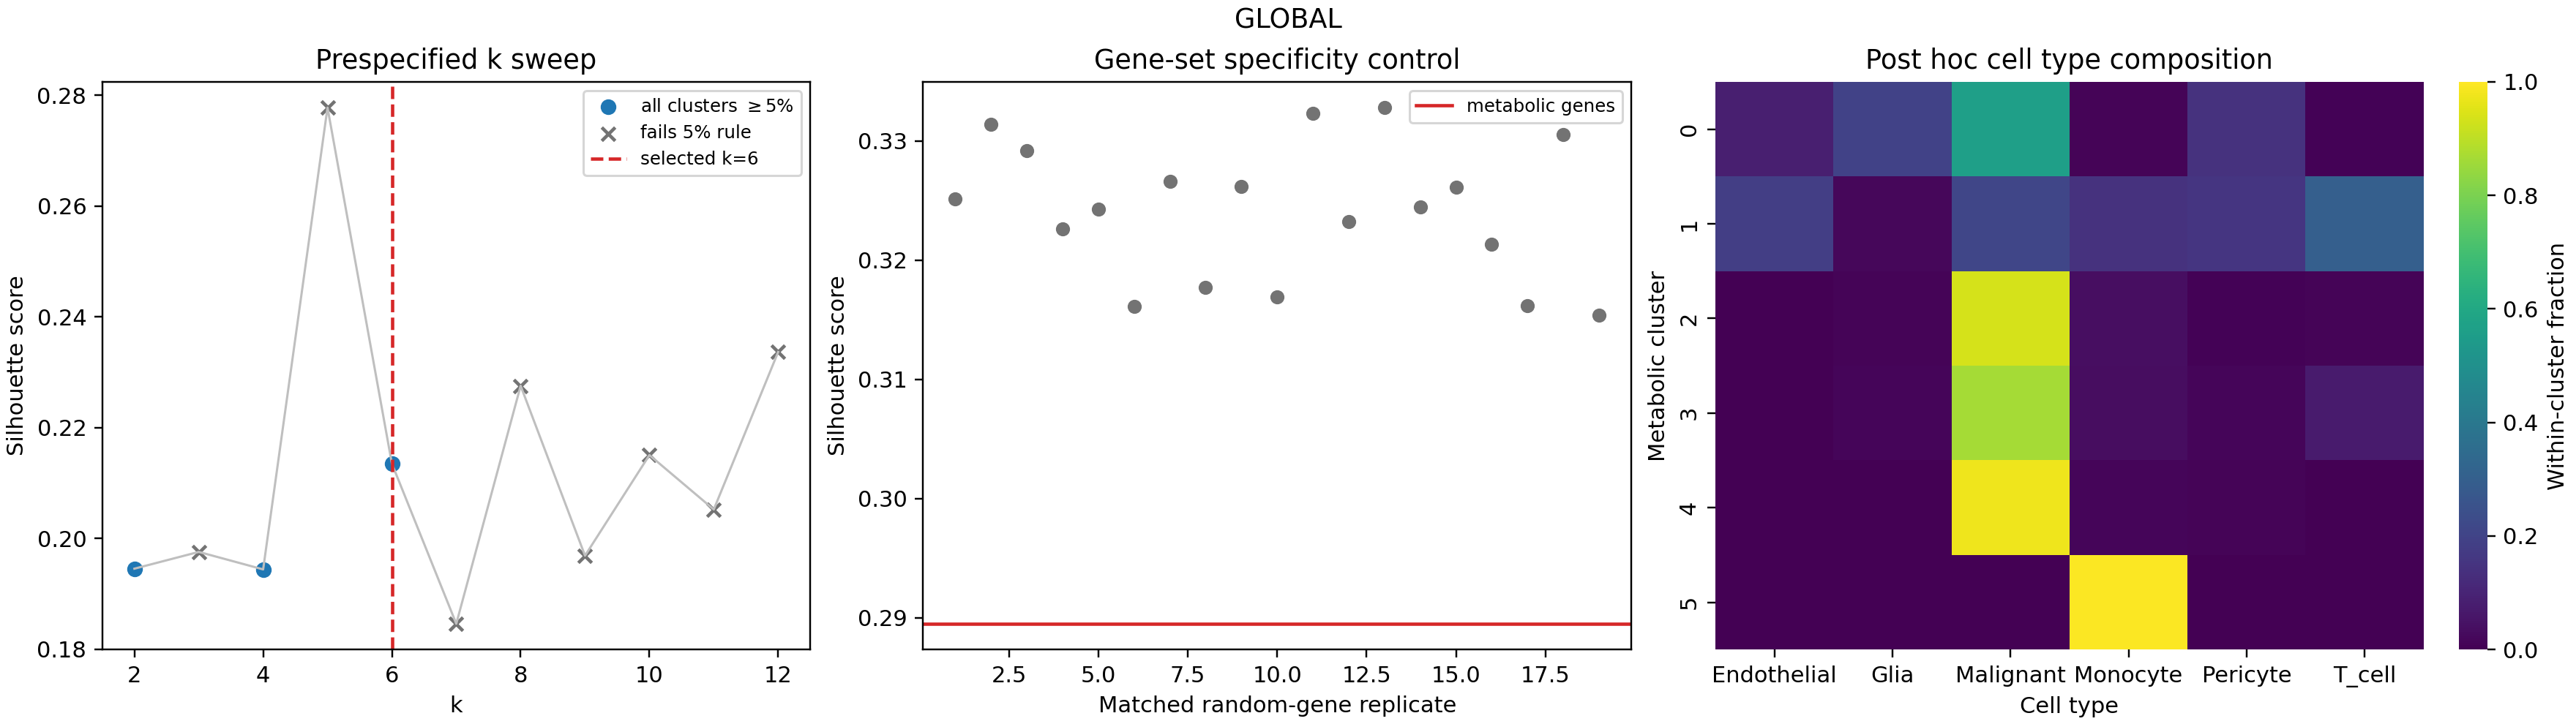
\includegraphics[width=\textwidth]{../figures/global_evidence.png}
\caption{Global evidence checks. Left: prespecified $k$ sweep; crosses fail the 5\% minimum-cluster rule, explaining why $k=6$ is reported instead of the higher-scoring but degenerate $k=5$. Middle: all 19 matched random non-metabolic gene sets exceed the metabolic control score. Right: post hoc cell-type composition of the six clusters.}
\label{fig:global-evidence}
\end{figure}

\subsection{Question 2: association with cell type}

There is a real descriptive association between the clusters and cell identity. NMI/AMI were 0.354/0.354 for broad cell type and 0.476/0.476 for cell subtype. Several clusters were strongly enriched: cluster 5 was 99.6\% monocyte; clusters 2 and 4 were 93.7\% and 97.4\% malignant, respectively. Cluster 1 was mixed, including 29.9\% T cells, 20.8\% malignant cells, 18.0\% endothelial cells, 15.4\% pericytes, and 14.2\% monocytes. Cluster 0 was 56.1\% malignant, 19.6\% glia, and 14.3\% pericyte.

\begin{table}[H]
\centering
\small
\begin{tabular}{lccp{0.48\textwidth}}
\toprule
Annotation & NMI & AMI & Interpretation \\
\midrule
Cell type & 0.354 & 0.354 & Descriptive association; no calibrated strength threshold \\
Cell subtype & 0.476 & 0.476 & Stronger, but subtype also reflects lineage and disease identity \\
Patient & 0.407 & 0.407 & Comparable to, and larger than, broad cell-type association \\
Sample & 0.361 & 0.361 & Comparable to cell type; samples are nested within patients \\
Source/region & 0.054 & 0.054 & Weak association in the pooled dataset \\
\bottomrule
\end{tabular}
\caption{Post hoc association metrics. Similar patient, sample, and cell-type values prevent a clean cell-type-specific metabolic interpretation.}
\end{table}

The association with cell type was visible within every patient but varied markedly: per-patient NMI ranged from 0.226 to 0.598. All six patients contained at least two global clusters at 5\% or more, which argues against a partition created by only one patient, but does not remove patient-dependent shifts. A further warning is transcript complexity: median detected-gene complexity ranged from 1,088.5 in cluster 3 to 5,481.5 in cluster 2, a 5.0-fold range. Normalization reduces library-size scale differences but cannot guarantee removal of complexity, cell-size, stress, dissociation, or copy-number-associated expression patterns.

Representative cluster-enriched genes also track known lineage programs: cluster 5 included \emph{TYMP}, \emph{SLCO2B1}, \emph{SLC11A1}, \emph{GLUL}, and \emph{ACSL1}; malignant-enriched clusters included glycolytic genes such as \emph{PKM}, \emph{GAPDH}, \emph{ENO1}, \emph{LDHA}, and \emph{LDHB}. These signatures are biologically interpretable, but they do not demonstrate discrete metabolic states independent of lineage.

\begin{figure}[H]
\centering
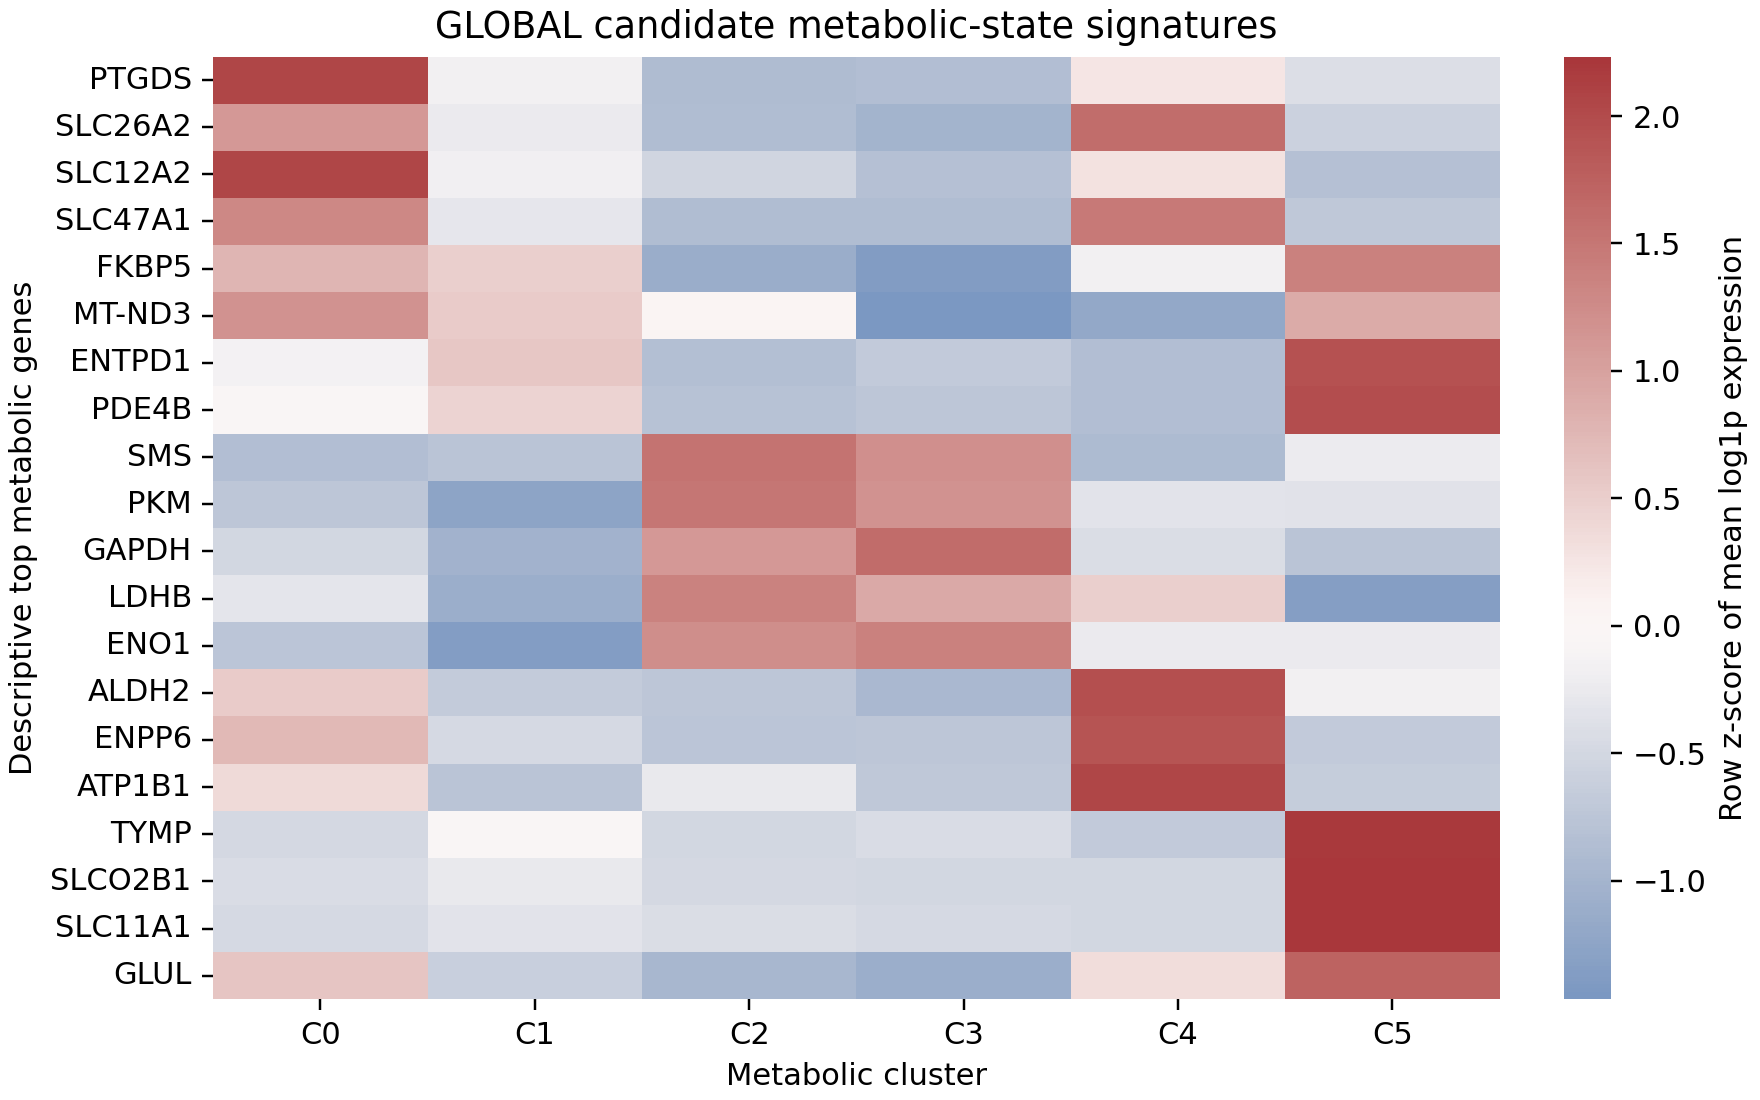
\includegraphics[width=0.93\textwidth]{../figures/global_signatures.png}
\caption{Descriptive global signatures. Values are row-wise $z$-scores of cluster mean $\log(1+x)$ expression for representative enriched metabolic genes. The heatmap is intended for labeling candidate patterns, not for inferential differential-expression claims.}
\label{fig:global-signatures}
\end{figure}

\subsection{Question 3: heterogeneity within CD8 T cells}

The exact 3CA subtype ``CD8 T cells'' contained 3,624 cells from all six patients. No solution from $k=2$ through $k=8$ had every cluster at or above 5\%; therefore there is no primary CD8 cluster solution under the prespecified rule. The best unconstrained $k=2$ result separated 54 cells (1.49\%) from 3,570 cells (98.51\%). Its full-data silhouette was high (0.633) and its ARI was 1.00 across the tested seeds, but this means the same rare outlier group is easy to recover; it does not make the group representative.

The rare group was highly patient-skewed: 45 of 54 cells were from patient 1, five from patient 4, and four from patient 5; patients 2, 3, and 6 contributed none. No patient contained both groups at 5\% or more. Median complexity was 8,384.5 detected genes in the rare group versus 1,182.0 in the main group, a 7.1-fold difference. Enriched symbols included \emph{PTGDS}, \emph{SLC26A2}, \emph{SLC47A1}, \emph{LYPLAL1}, \emph{EPHX1}, \emph{ENPP6}, \emph{GLUL}, \emph{ALDH2}, \emph{SLC4A4}, and \emph{PRDX2}. Their magnitude, high complexity, and concentration in patient 1 make annotation contamination, doublets, anatomical carry-over, or another high-RNA subgroup plausible alternatives to a CD8 metabolic state.

On the control subsample, the metabolic score was 0.665 and none of 19 matched random lists exceeded it, giving the minimum attainable add-one value of 0.05. This does not rescue the claim: the cluster violates the size rule, was found by optimizing $k$, lacks patient-level replication, and has a major complexity imbalance. It is an audit target, not a validated state.

\begin{figure}[H]
\centering
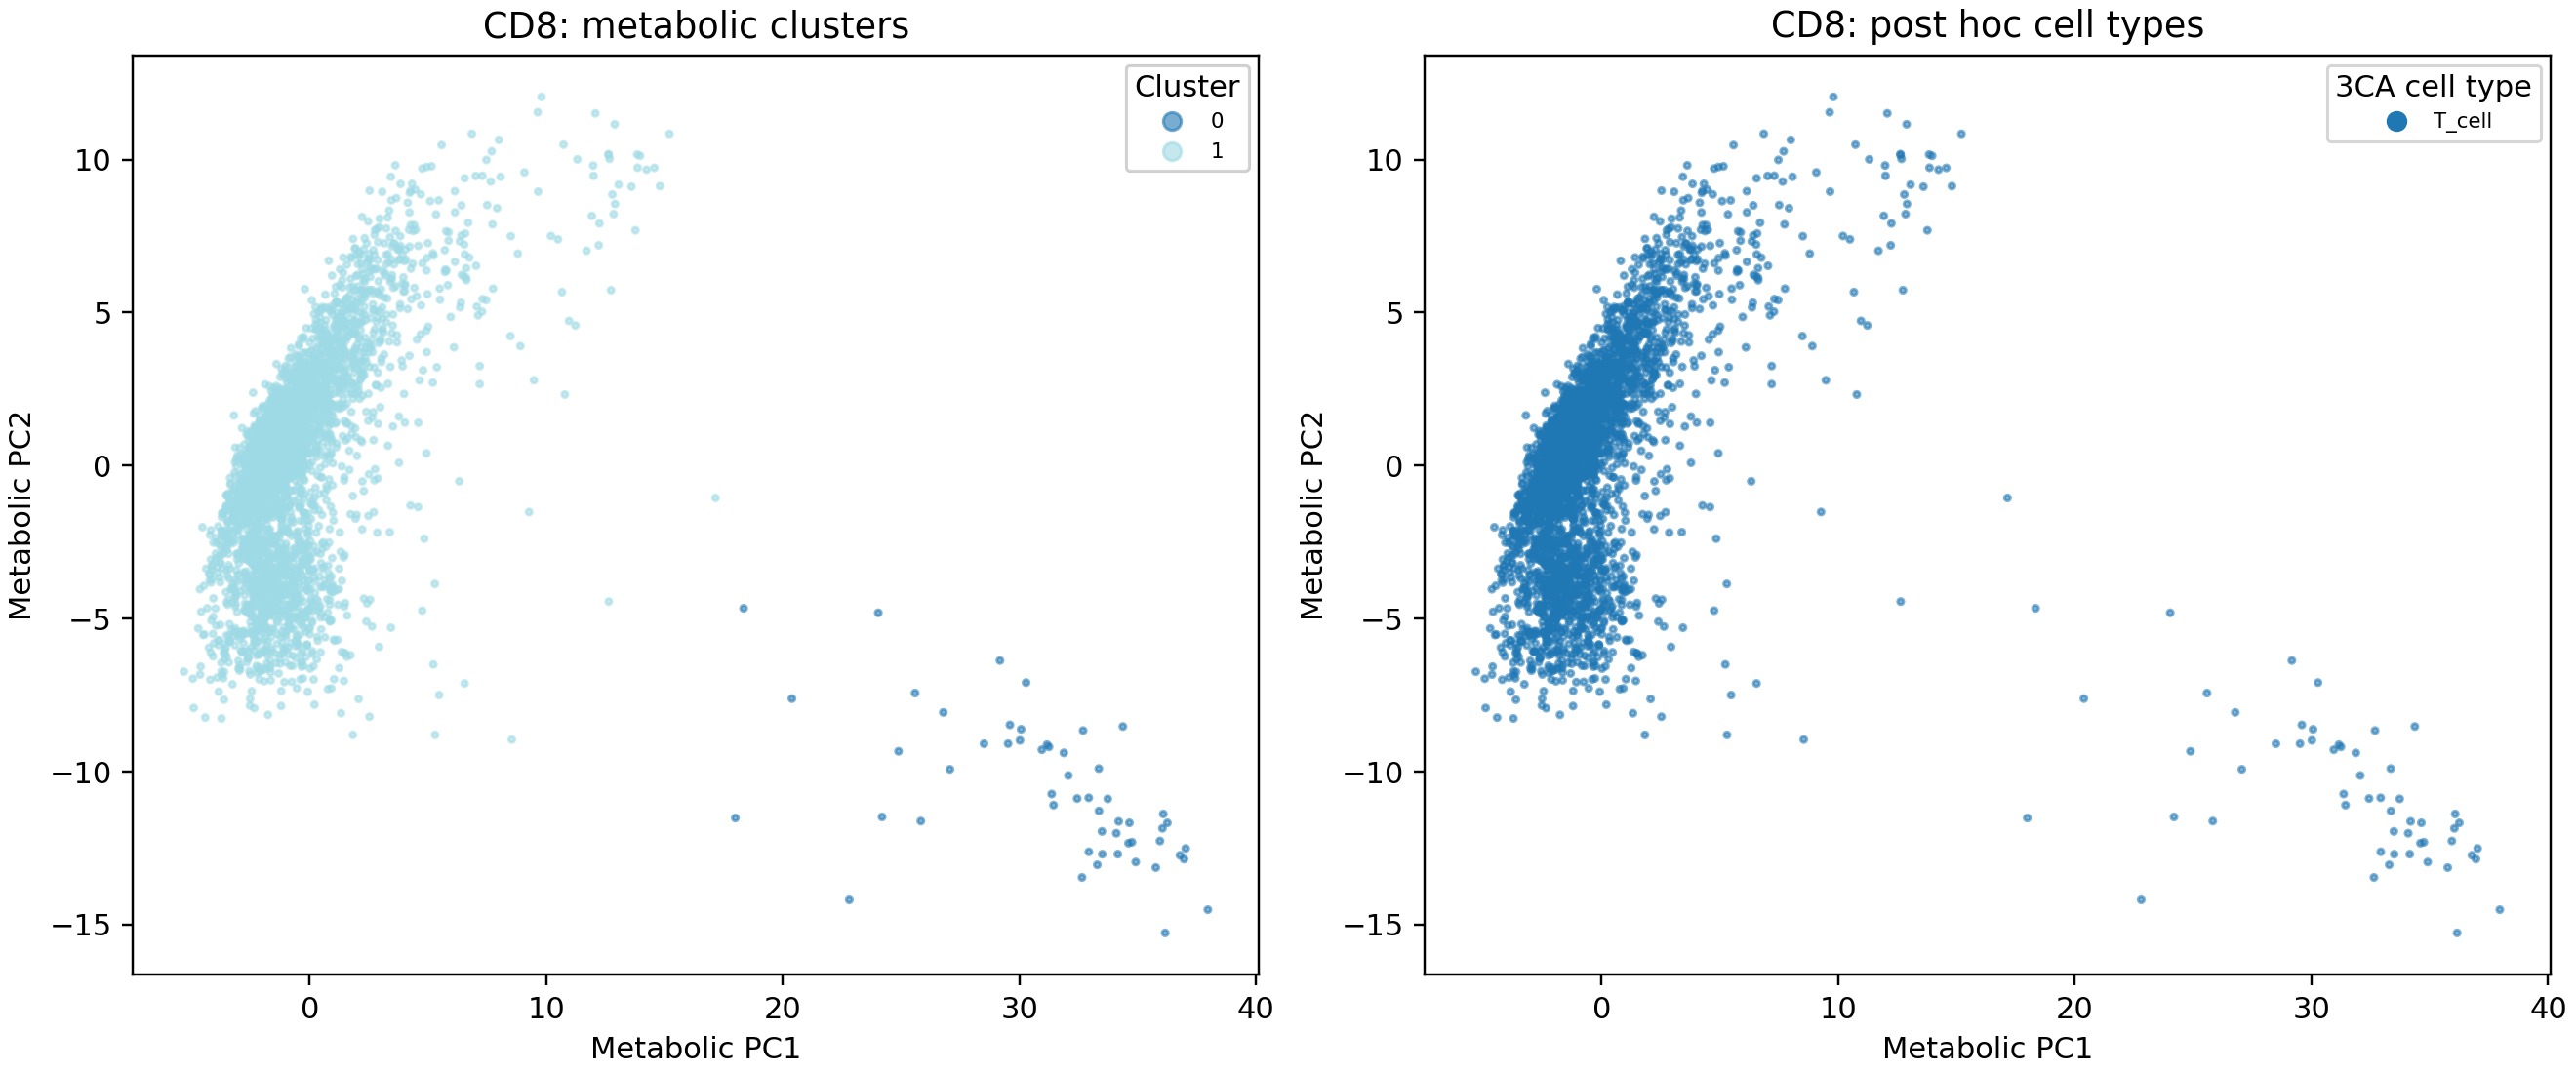
\includegraphics[width=\textwidth]{../figures/cd8_embedding.png}
\caption{CD8 diagnostic PCA. The apparent split is a small, distant group of 54 cells rather than two broadly represented populations. Both panels contain only cells annotated by 3CA as CD8 T cells.}
\label{fig:cd8-embedding}
\end{figure}

\begin{figure}[H]
\centering
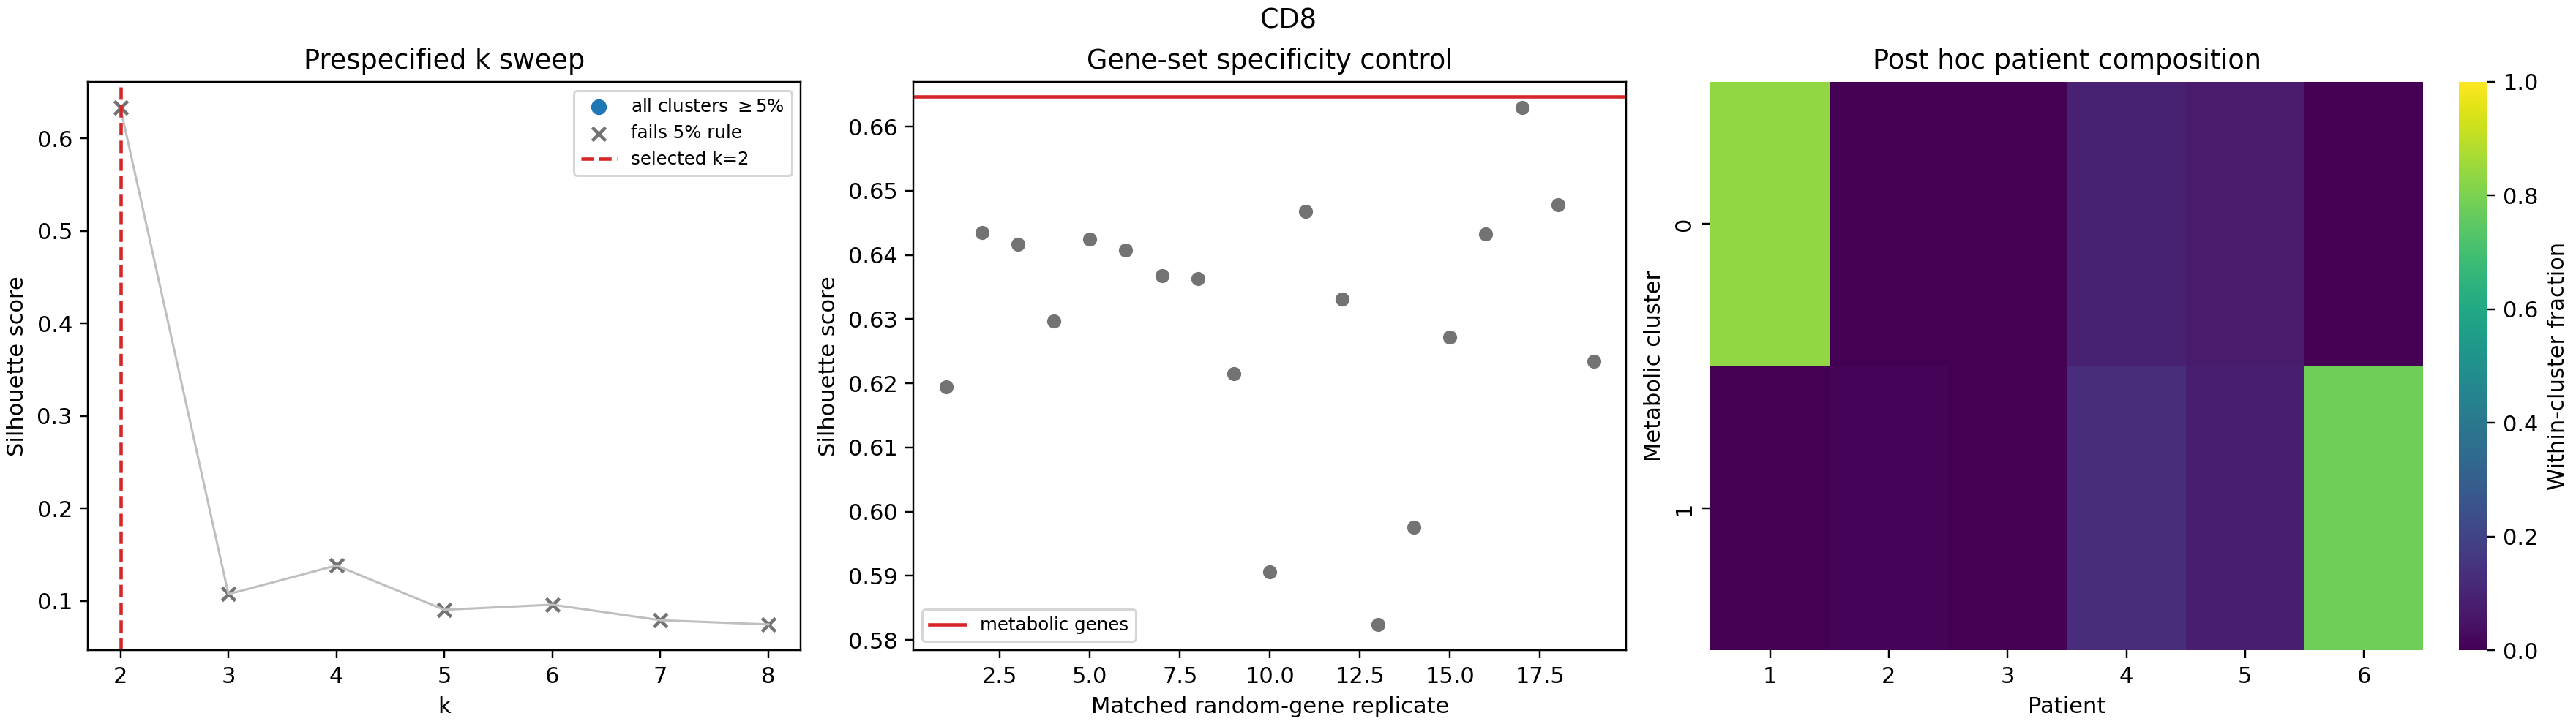
\includegraphics[width=\textwidth]{../figures/cd8_evidence.png}
\caption{CD8 evidence checks. Left: every tested $k$ fails the 5\% size rule. Middle: exploratory matched-gene control; the red line is the metabolic score. Right: patient composition, showing that 45 of 54 rare-group cells are from patient 1.}
\label{fig:cd8-evidence}
\end{figure}

\begin{figure}[H]
\centering
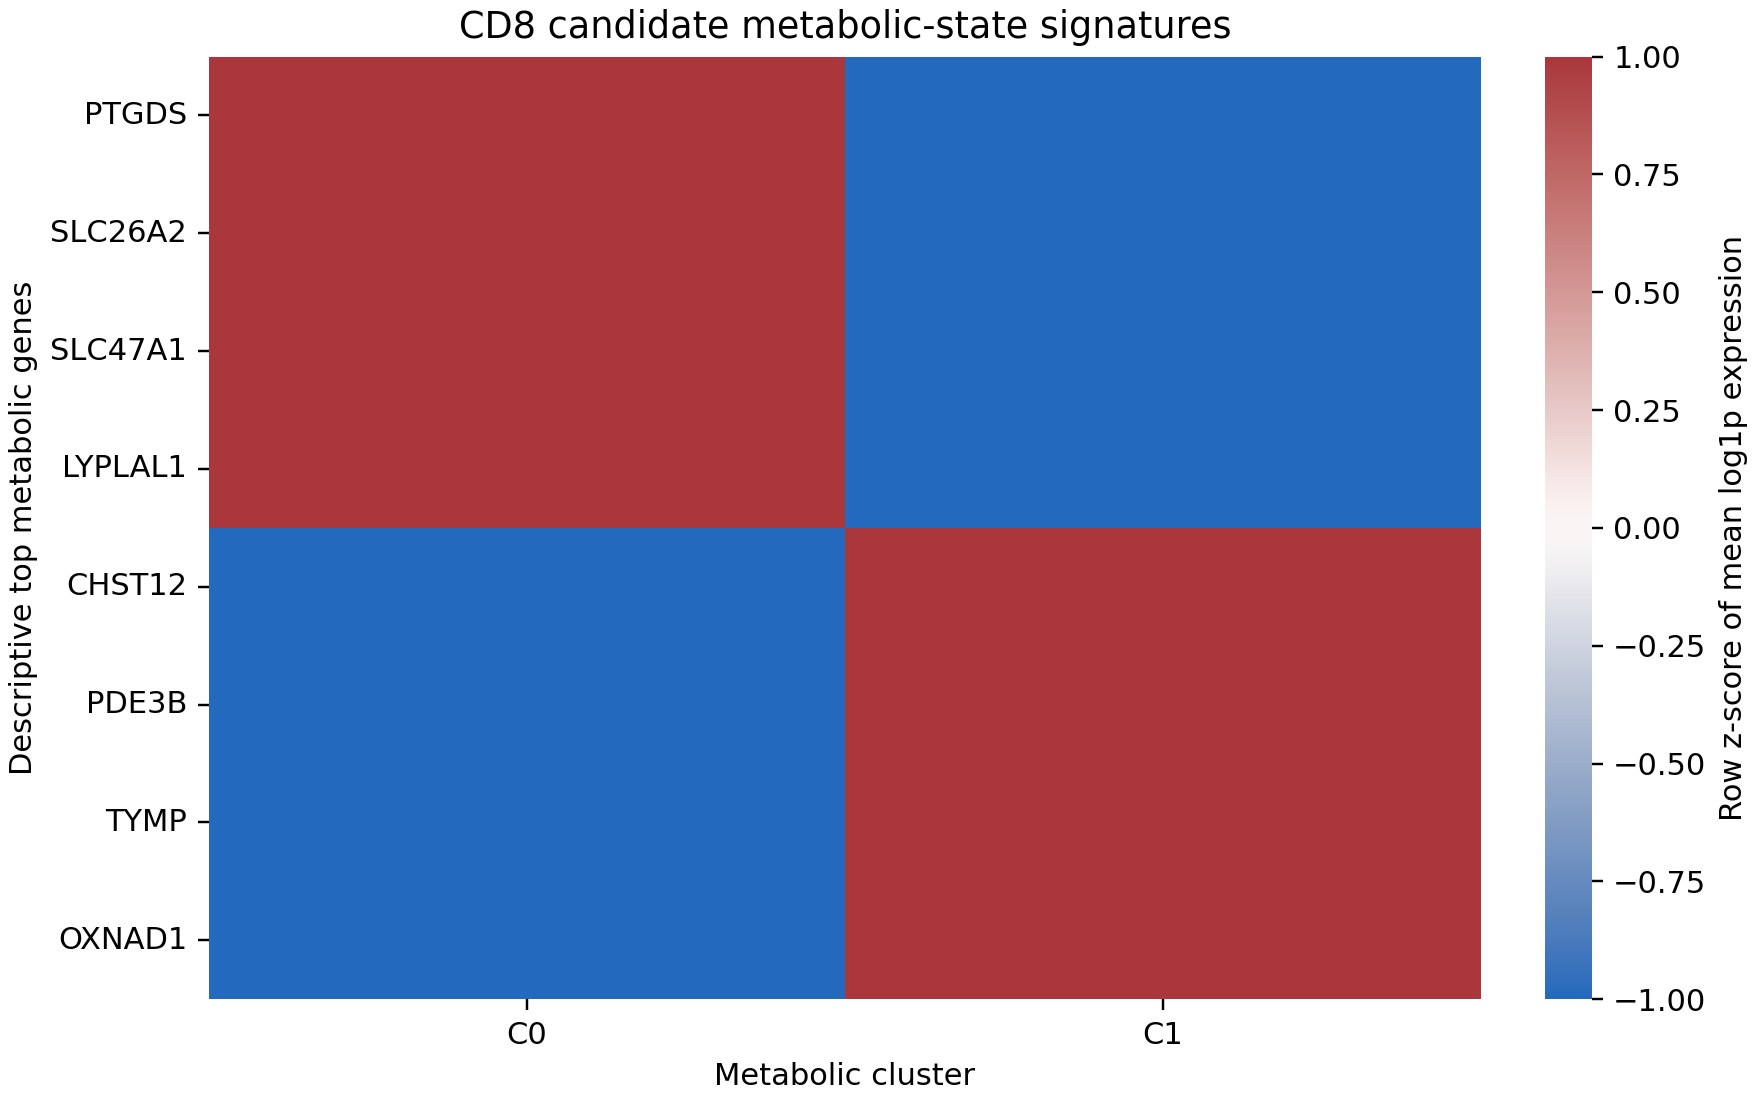
\includegraphics[width=0.88\textwidth]{../figures/cd8_signatures.png}
\caption{Diagnostic CD8 signatures. The two-column heatmap necessarily accentuates the contrast and should not be read as evidence that the 54-cell group is a general CD8 state.}
\label{fig:cd8-signatures}
\end{figure}

\section{Interpretation and limitations}

\begin{enumerate}
\item \textbf{Transcription is not metabolic flux.} scRNA-seq measures RNA abundance, not enzyme activity, substrate availability, redox state, or pathway flux. The phrase ``metabolic state'' here means a candidate transcriptional state defined by genes on the supplied list.
\item \textbf{Only one cancer study was analyzed.} The design avoids cross-study batch effects but limits generalizability to meningioma and provides only six independent patients. A pan-cancer conclusion requires locked analysis choices and validation across independent studies or patient-level pseudo-bulk summaries.
\item \textbf{The user list is broad.} It contains transporters, housekeeping enzymes, mitochondrial genes, signaling regulators, and genes with strong lineage expression. Expression-matched random controls show that a large, expressed gene set can cluster cells even when it is not specifically metabolic.
\item \textbf{Cluster selection is exploratory.} Silhouette optimization and multiple tested $k$ values favor discoverable structure. The 5\% rule limits one failure mode but does not turn an exploratory analysis into confirmation.
\item \textbf{Cell annotations and quality require audit.} The CD8 rare group should be checked for doublet scores, canonical T-cell markers, ambient RNA, mitochondrial fraction, sample-processing metadata, and anatomical origin before any biological label is assigned. Those fields were not all available in the exported 3CA metadata.
\item \textbf{No cell-level inferential $P$-values are reported.} Cells are not independent biological replicates. The 19-control empirical values are calibration summaries with coarse resolution, not patient-level tests.
\end{enumerate}

\section{Conclusion}

The workflow answers the computational part of the request: the supplied metabolic genes can generate clusters in the selected 3CA single-cell dataset. The evidence does \emph{not}, however, support the stronger biological statement that these are distinct metabolism-specific states. Globally, cell type is associated with the partition, but patient, sample, transcript complexity, and generic expressed-gene structure are equally important competing explanations. Within CD8 T cells, the only strong split is a 54-cell, high-complexity, patient-skewed outlier group that fails the prespecified prevalence and replication criteria.

A defensible next validation would freeze the preprocessing, feature list, size rule, and $k$ strategy; audit/remove doublets and non-T-like CD8 cells; then test patient-level state scores or label transfer in independent 3CA studies. Until that is done, the six global clusters and two CD8 diagnostic groups should be called \emph{candidate transcriptional groupings}, not metabolic states.

\section{Reproducibility and output map}

The complete analysis is contained in one Python script with an executable self-test:
\begin{itemize}
\item \path{code/analyze_metabolic_states.py}: preprocessing, PCA, clustering, guardrail, stability, matched-gene controls, annotation metrics, tables, and figures.
\item \path{results/results_summary.json}: machine-readable headline results and environment versions.
\item \path{results/metabolic_genes_matched.csv} and \path{results/metabolic_genes_unmatched.csv}: gene mapping audit.
\item \path{results/global_*} and \path{results/cd8_*}: $k$ sweeps, cell assignments, controls, compositions, diagnostics, and signatures.
\item \path{figures/}: all figures used in this report.
\end{itemize}

The script was executed with Python 3.12.4, NumPy 1.26.4, pandas 2.2.2, SciPy 1.14.0, scikit-learn 1.5.1, Matplotlib 3.10.1, and seaborn 0.13.2. The exact archive and gene-list hashes above make input identity auditable.

\section*{Sources}

\begin{enumerate}
\item Weizmann Curated Cancer Cell Atlas (3CA), homepage: \url{https://www.weizmann.ac.il/sites/3CA/}; study/category page: \url{https://www.weizmann.ac.il/sites/3CA/brain}. Accessed 14 September 2026.
\item 3CA methods: \url{https://www.weizmann.ac.il/sites/3CA/methods}. Accessed 14 September 2026.
\item Choudhury \emph{et al.}, \emph{Nature Genetics} (2022), source article linked by 3CA: \url{https://www.nature.com/articles/s41588-022-01061-8}.
\end{enumerate}

\end{document}
